\documentclass[border=4pt]{standalone}
\usepackage{amsmath}
\usepackage{tikz}
\usetikzlibrary{arrows.meta,calc,decorations.markings,shadings}
\begin{document}
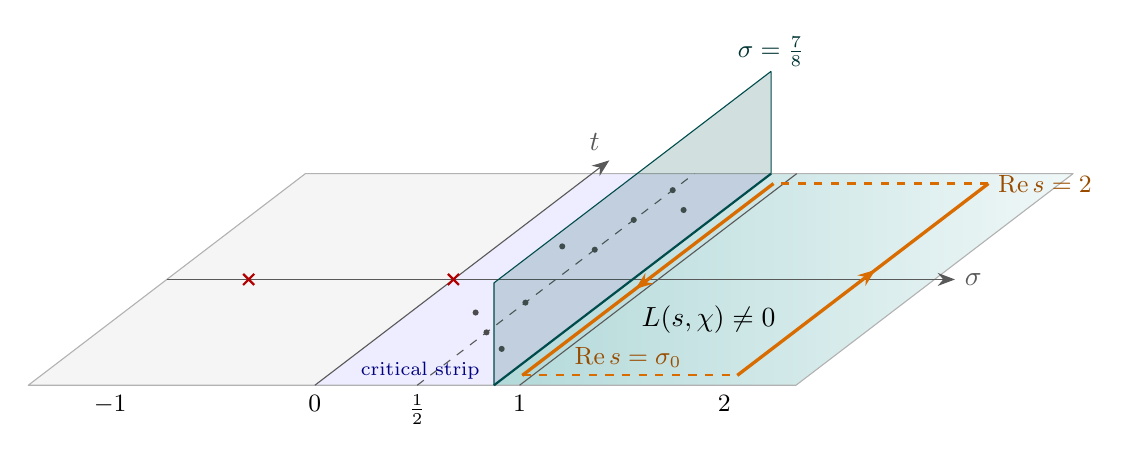
\begin{tikzpicture}[
  x={(2.6cm,0cm)}, y={(0.55cm,0.42cm)}, z={(0cm,1cm)},
  >={Stealth[length=2.2mm]}, line join=round]
  % base plane
  \def\tl{-3.2}\def\th{3.2}
  \fill[gray!8] (-1.4,\tl,0)--(0,\tl,0)--(0,\th,0)--(-1.4,\th,0)--cycle;
  \fill[blue!7] (0,\tl,0)--(0.875,\tl,0)--(0.875,\th,0)--(0,\th,0)--cycle;
  \shade[left color=teal!30,right color=teal!6] (0.875,\tl,0)--(2.35,\tl,0)--(2.35,\th,0)--(0.875,\th,0)--cycle;
  \draw[gray!60] (-1.4,\tl,0)--(2.35,\tl,0)--(2.35,\th,0)--(-1.4,\th,0)--cycle;
  % axes
  \draw[->,gray!70!black] (-1.4,0,0)--(2.45,0,0) node[right]{$\sigma$};
  \draw[->,gray!70!black] (0,\tl,0)--(0,\th+0.4,0) node[above left]{$t$};
  \draw[gray!70!black,dashed] (0.5,\tl,0)--(0.5,\th,0);
  \draw[gray!70!black] (1,\tl,0)--(1,\th,0);
  \foreach \s/\lab in {-1/{-1},0/0,0.5/{\tfrac12},1/1,2/2}
    \node[below,font=\small] at (\s,\tl,0) {$\lab$};
  % zeros allowed only on the left of 7/8
  \foreach \yy/\xx in {-1.6/0.5,-0.7/0.5,0.9/0.5,1.8/0.5,2.7/0.5,
                       -2.1/0.68,2.1/0.68,-1.0/0.32,1.0/0.32}
    \fill[black!70] (\xx,\yy,0) circle (1.1pt);
  % poles of x^s/(s(s+1))
  \foreach \s in {-1,0}
    \draw[red!70!black,thick] ($(\s,0,0)+(-2pt,-2pt)$)--($(\s,0,0)+(2pt,2pt)$)
          ($(\s,0,0)+(-2pt,2pt)$)--($(\s,0,0)+(2pt,-2pt)$);
  % translucent wall at sigma = 7/8
  \fill[teal!60!black,opacity=0.18] (0.875,\tl,0)--(0.875,\th,0)--(0.875,\th,1.3)--(0.875,\tl,1.3)--cycle;
  \draw[teal!60!black,thick] (0.875,\tl,0)--(0.875,\th,0);
  \draw[teal!60!black] (0.875,\tl,1.3)--(0.875,\th,1.3) (0.875,\tl,0)--(0.875,\tl,1.3) (0.875,\th,0)--(0.875,\th,1.3);
  \node[teal!40!black,font=\small] at (0.875,\th,1.55) {$\sigma=\tfrac78$};
  % contour: line Re s = 2 moved to Re s = sigma_0
  \def\so{0.95}
  \draw[orange!85!black,very thick,postaction={decorate},
        decoration={markings,mark=at position 0.55 with {\arrow{>}}}]
        (2,\tl+0.3,0)--(2,\th-0.3,0);
  \draw[orange!85!black,very thick,postaction={decorate},
        decoration={markings,mark=at position 0.55 with {\arrow{>}}}]
        (\so,\th-0.3,0)--(\so,\tl+0.3,0);
  \draw[orange!85!black,thick,dashed] (2,\th-0.3,0)--(\so,\th-0.3,0) (\so,\tl+0.3,0)--(2,\tl+0.3,0);
  \node[orange!60!black,font=\small,right] at (2,\th-0.3,0) {$\operatorname{Re}s=2$};
  \node[orange!60!black,font=\small] at (1.35,\tl+0.85,0) {$\operatorname{Re}s=\sigma_0$};
  % labels of the regions
  \node[align=center] at (1.5,-1.2,0) {$L(s,\chi)\neq0$};
  \node[font=\scriptsize,blue!50!black] at (0.42,\tl+0.45,0) {critical strip};
\end{tikzpicture}
\end{document}
